\chapter{Materials Preparation and Analysis}

In this chapter we discuss methods used to prepare and analyze the thin film oxides as well as provide a short review on the theory of dielectrics. 

\section{The dielectric properties of materials}
\subsection{Insulating materials and charge}

Capacitors come in various shapes and sizes, the simplest configuration being the parallel plate capacitor (PPC). The PPC is comprised of an insulating material that is sandwiched between two conducting terminals (Figure \ref{fig:PPC}a). If we consider a PPC in a vacuum with only space between the two terminals connected to a battery, the capacitance between the terminals is:
\begin{equation} \label{eq:capfreespace}
C_{o} = \frac{Q_{o}}{V}.
\end{equation}
Here, $C_{o}$ is the capacitance of the parallel plate capacitor in free space, $Q_{o}$ is the charge on the terminals, and $V$ is the voltage that is applied between the terminals. Now, if we slide an insulating material between the two terminals as shown in Figure \ref{fig:PPC}b,
\begin{figure}[t]
	\centering
	\begin{subfigure}[b]{\linewidth}\centering
	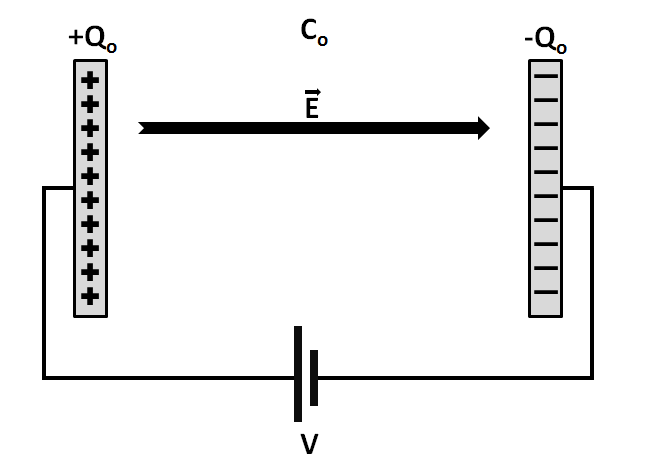
\includegraphics[width=.7\linewidth]{chapter_2/cap1}
	\caption{}\label{fig:sub1}
	\end{subfigure}\
	\begin{subfigure}[b]{\linewidth}\centering
	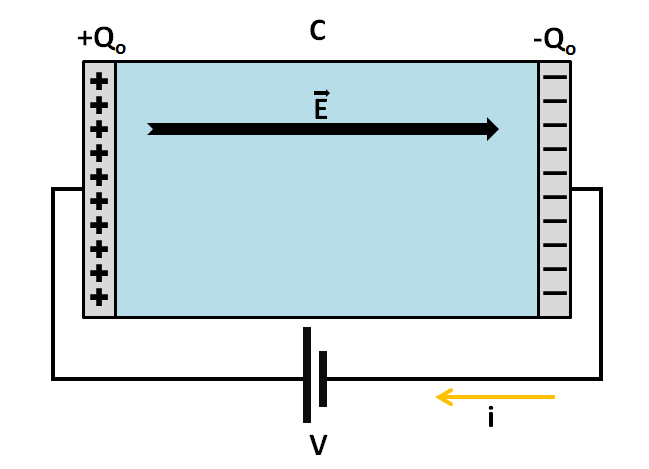
\includegraphics[width=.7\linewidth]{chapter_2/cap2}
	\caption{}\label{fig:sub2}
	\end{subfigure}
	\caption{(a) Parallel plate capacitor in a vacuum connected to a battery with voltage V and capacitance C$_{o}$. (b) The capacitance changes from C$_{o}$ to C when an insulating material is placed between the terminals. }
	\label{fig:PPC}
\end{figure}
current would immediately flow through the external circuit resulting in an increased amount of separated charge. The new charge at the two terminals is now $Q$ such that the capacitance changes to $C$, so equation \ref{eq:capfreespace} is slightly modified to
\begin{equation} \label{eq:capreal}
C = \frac{Q}{V}.
\end{equation}
The ratio between the initial and final charge stored in the capacitor is the relative dielectric constant $\varepsilon_{r}$ (also written as $\kappa$ or $k$) 
\begin{equation}
\frac{Q}{Q_{o}} = \varepsilon_{r}
\end{equation}
and alternatively, the ratio between the two capacitances
\begin{equation}\label{eq:cap0}
\frac{C}{C_{o}}=\varepsilon_{r}.
\end{equation}
This simple example shows that dielectrics are essentially charge storage devices and that the dielectric constant is a  parameterization of how effectively a material is able to store charge. Due to its simplicity, many modern electronics exploit the parallel plate configuration. One thing to note is that due to finite size effects the field lines that go from one side of the terminal to the other, especially on the periphery of the terminals, are not perfectly straight lines (Figure \ref{fig:cap3}).

\begin{figure}[t]
	\centering
	\begin{subfigure}[b]{\linewidth}\centering
	\centering
	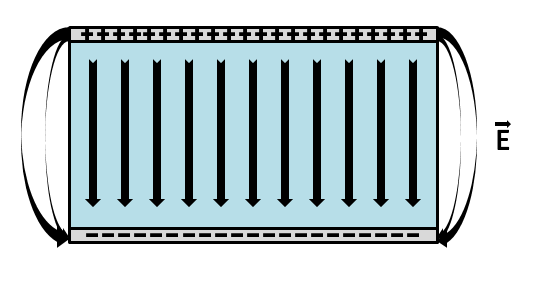
\includegraphics[width=0.7\linewidth]{chapter_2/cap3}
	\caption{}\label{fig:cap3}
	\end{subfigure}
	\begin{subfigure}[b]{\linewidth}\centering
	\centering
	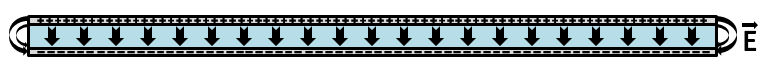
\includegraphics[width=0.7\linewidth]{chapter_2/cap4}
	\caption{}\label{fig:cap4}
\end{subfigure}

\caption{The contribution of the fringing field to the total electric field changes with the aspect ratio of the capacitor. Thin film capacitors have a large aspect ratio so the contribution of the fringing field is minimal.}
\end{figure}

Field lines at the outer edges of the capacitor---so-called fringing fields---are not entirely contained between the plates. For our devices we assume that these fringing fields do not contribute significantly to the electrical measurement owing to the large aspect ratio between the thickness of the insulating film (d)---ranging from $\sim$10 to several 100 nanometers---and the width of the capacitors (w) (several hundred microns) in our devices, which allows us to greatly simplify the integral equation of Gauss's law. For a capacitor with no dielectric, 
\begin{equation}\label{eq:gauss_law}
\oiint_{S}\vec{\textbf{E}}\cdot d\vec{\textbf{A}} = E_{o}A= \frac{Q_{o}}{\varepsilon_{o}}
\end{equation} 
in which $E_{o}$ is the electric field between the two plates, $A$ is the area of the capacitor, and $\varepsilon_{o}$ is the permittivity of free space. Combining with equation \ref{eq:capfreespace}, rearranging, and from the fact that $E_{o} = Vd$, we can relate the capacitance to the applied electric field,
\begin{equation}\label{eq:cap1}
\frac{\varepsilon_{o}AE_{o}}{V} = \frac{\varepsilon_{o}A}{d} =C_{o}.
\end{equation}
Recall, that for a capacitor with an insulating material the capacitance is larger by a constant factor $\varepsilon_{r}$
\begin{equation}
\label{eq:cap2}
C = \frac{\varepsilon_{o} \varepsilon_{r} A}{d}.
\end{equation}
Equation \ref{eq:cap2} illustrates the dependence of capacitance on geometry, namely capacitance area and distance between plates, and intrinsic electronic properties through $\varepsilon_{r}$. Our study focuses on the composition dependence of $\varepsilon_{r}$ for amorphous dielectric oxides. Thus, we introduce the concept of dielectric polarization to describe their intrinsic properties. 

\subsection{Polarization}

As we saw earlier, inserting a dielectric between two electrical terminals changes the capacitance between the two terminals. This is a result of the atoms in the dielectric spontaneously polarizing in order to align with the electric field. \textit{Classically}, the spontaneous polarization of the atoms can be represented as a chain of positive and negative point charges that connect head to tail (Figure \ref{cap5}).
\begin{figure}
\centering
\noindent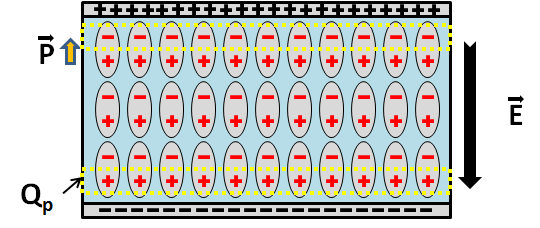
\includegraphics[width=0.7\linewidth]{chapter_2/cap5}
\caption{Application of an external electric field causes the atoms in the material to polarize along the direction of the applied field. Consequently, a surface polarization charge $Q_{p}$ forms at the interface between the electrode and the dielectric.}
\label{cap5}
\end{figure}
The polarization of the atoms within the material in turn causes the surface of the dielectric to polarize, forming a \textit{surface polarization} charge $Q_{p}$. We can consider the surface polarization charge to be a single dipole moment $p$ across the dielectric. We define polarization to be the total dipole moment per volume, which is equivalently represented as a \textit{surface polarization charge density} $\sigma_{p}$
\begin{equation}\label{eq:polarization}
P = \frac{p}{V} = \frac{Q_{d}d}{Ad} = \frac{Q_{p}}{A} = \sigma_{p}.
\end{equation}
To compensate for the new charge $Q_{p}$ that has formed on the surface of the dielectric, current flows through the external circuit (recall Figure \ref{fig:PPC}b). As a result, the free surface charge $Q_{o}$ becomes $Q$. The total charge on the plates can be  expressed as
\begin{equation}\label{eq:totalcharge}
Q = Q_{o} + Q_{p}.
\end{equation}

If we divide equation \ref{eq:totalcharge} by the area of the capacitor $A$, we can rewrite equation \ref{eq:totalcharge} in terms of charge densities $\sigma$
\begin{equation}\label{eq:charged}
\sigma = \sigma_{o}+\sigma_{p}.
\end{equation}
From equation \ref{eq:polarization} we know that $\sigma_{p}$ is the surface polarization density and $\sigma_{o}$ is just the \textit{free surface charge density}. The free surface charge density can be written in terms of the electric field, $E$ by rearranging equation \ref{eq:gauss_law}
\begin{equation}\label{eq:charge2}
\sigma = \varepsilon_{o}E + \sigma_{p}.
\end{equation}
Substituting $P$ for $\sigma_{p}$ and since $P = \chi_{e}\varepsilon_{o}E$ we get 
\begin{equation}\label{eq:charge3}
\frac{\sigma}{E } = \varepsilon_{o}(1+\chi_{e})
\end{equation}
where $\chi_{e}$ is the electric susceptibility. Finally, we can relate equation \ref{eq:charge3} back to capacitance 
\begin{equation}\label{eq:charge4}
\frac{\sigma}{E } = \frac{Q}{AE} = \frac{Cd}{A} = \varepsilon_{o}(1+\chi_{e})
\end{equation}
\begin{equation}\label{eq:charge5}
C = \frac{\varepsilon_{o}(1+\chi_{e})A}{d} =  \frac{\varepsilon_{o} \varepsilon_{r} A}{d} 
\end{equation}
so $(1+\chi_{e})= \varepsilon_{r}$.

The simple relation between relative permittivity, capacitance, and susceptibility suggests that measuring the capacitance of the PPC reveals information about the polarization of atoms. For instance, if a polarizable medium did not exist between the conducting terminals (vacuum) $\chi_{e} =  0$, we would be left with equation \ref{eq:cap1}. On the other hand, when an polarizable (e.g. insulator) material was present $\chi_{e} > 0$, the capacitance would be greater by a constant $\varepsilon_{r}$.

\subsection{Local field, Clausius-Mossotti, and polarizability}

We have made the point that macroscopic dielectric properties have microscopic origins. We develop this concept further by establishing a connection between the dielectric constant and polarizability of the atom. 

As mentioned earlier, when an electric field $\textbf{E}_{o}$ is applied to a dielectric the atoms polarize to align with the field. However, the electric field felt by each atom---the ``local field" ($\textbf{E}_{\text{loc}}$)---is in fact different from the externally applied field, $\textbf{E}_{o}$. We calculate the local field by cutting out a hypothetical cavity in the material centered at $i$, and removing atom $i$ (the atom cannot produce its own field) as shown in Figure \ref{depfield}.

\begin{figure}
\centering
\noindent
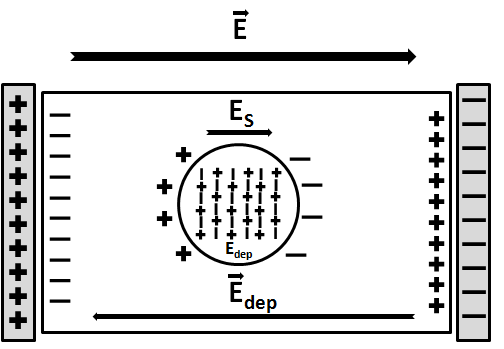
\includegraphics[width=0.7\textwidth]{chapter_2/depfield}
\caption{To calculate the local field felt by the atom inside the material we create a hypothetical cavity in the material, creating a uniformly polarized sphere. The local field is determined by summing all the contributions to the local field.}
\label{depfield}
\end{figure}

The local field at atom $i$ is determined by summing the different contributions to the local field. The contributions from outside of the cavity $\textbf{E}(\textbf{r})$ equal the difference between the applied field and the depolarization field $\textbf{E} = \textbf{E}_{o} - \textbf{E}_{dep}$. Within the cavity we have contributions from $\textbf{E}_{\text{sphere}}(\textbf{r})$, which is the macroscopic field inside a uniformly polarized sphere, and local dipolar contributions of the atoms within the cavity, $\textbf{E}_{\text{dipolar}}(\textbf{r})$. We write $\textbf{E}_{\text{loc}}(\textbf{r})$ as
\begin{equation}\label{eq:local}
\textbf{E}_{\text{loc}}(\textbf{r}) = \textbf{E}(\textbf{r}) + \textbf{E}_{\text{sphere}}(\textbf{r}) + \textbf{E}_{\text{dipolar}}(\textbf{r}).
\end{equation}

From electrostatics, we know that $\textbf{E}_{\text{sphere}}(\textbf{r})$ is $4\pi\textbf{P}(\textbf{r})/3$, where $\textbf{P}(\textbf{r})$ is the polarization density defined as \textbf{P} $(\textbf{r}) = \textbf{p}(\textbf{r})/\textit{v}$, that is, polarization per unit volume. Equation \ref{eq:local} is further simplified for high symmetry materials. For these materials, e.g. cubic and amorphous materials, we assume that dipolar term, $\textbf{E}_{\text{dipolar}}(\textbf{r})$ vanishes. Now, the local field is 
\begin{equation}\label{eq:local2}
\textbf{E}_{\text{loc}}(\textbf{r}) = \textbf{E}(\textbf{r}) + \frac{4\pi\textbf{P}(\textbf{r})}{3}.
\end{equation}

The following,
\begin{equation}\label{eq:disp}
\textbf{D}(\textbf{r}) = \varepsilon\textbf{E}(\textbf{r})
\end{equation}
relates the electric displacement $\textbf{D}(\textbf{r})$ to the dielectric constant $\varepsilon$. Using Equations \ref{eq:local2} and \ref{eq:disp}, we can express $\textbf{P}(\textbf{r})$ in terms of $\textbf{E}(\textbf{r})$
\begin{equation}\label{eq:disp2}
\textbf{P}(\textbf{r}) = \frac{\varepsilon - 1}{4\pi}\textbf{E}(\textbf{r}).
\end{equation}
Combining Equation \ref{eq:local2} and \ref{eq:disp2} eliminates $\textbf{P}(\textbf{r})$ and becomes an equation that links the local electric field $\textbf{E}_{\text{loc}}(\textbf{r})$ to measurable quantities
\begin{equation}
\textbf{E}^{\text{loc}}(\textbf{r}) = \frac{\varepsilon + 2}{3}\textbf{E}(\textbf{r}).
\label{eq:eloc}
\end{equation}
Polarization of the atom is related to the polarizability and local field by $\textbf{p}(\textbf{r}) = \alpha\textbf{E}_{\text{loc}}(\textbf{r})$. Recalling that $\textbf{P}(\textbf{r}) = \textbf{p}(\textbf{r})/v$, we can use Equation \ref{eq:disp2} and \ref{eq:eloc} to obtain the Claussius-Mossotti equation 
\begin{equation}
\frac{\varepsilon - 1}{\varepsilon + 2} = \frac{4\pi\alpha}{3v}.
\label{eq:CM}
\end{equation}
The Claussius-Mossotti (CM) equation is a much used equation that relates a local property---polarizability, $\alpha$---to a macroscopic property, the dielectric constant. 

In actuality, the situation is a bit more subtle. A more thorough investigation of the phenomena of polarization reveals the ambiguity of assigning individual dipole moments to atoms and the choice of a proper primitive cell, known as the polarization ambiguity. There have recently been several theoretical developments that have led to sophisticated methods allowing researchers to calculate the spontaneous polarization of periodic solids \cite{Spaldin2012}. However, the aperiodicity of amorphous materials still poses a theoretical and computational challenge due to the lack of long range ordering. In this study, we merely rely on the CM equation as a way to experimentally extract trends in how polarizability (a local property) changes as a function of concentration. 

\subsection{Frequency dependence}

The process of polarization is an inherently frequency dependent process. Different polarizability mechanisms are accessible at different frequencies and give rise to the dispersive behavior of the dielectric constant (Figure \ref{fig:polardisp}).

\begin{figure}[ht]
\centering
\noindent
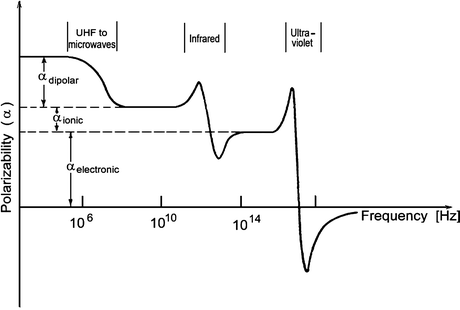
\includegraphics[width=0.7\linewidth]{chapter_2/polarizabilitydispersion}
\caption{Dispersion relation of polarizability as a function of frequency. Figure taken from reference \cite{Subhadra2011}.}
\label{fig:polardisp}
\end{figure}

For dielectric materials that are presented in this study, the components that contribute to the dielectric constant are mainly electronic ($\alpha_{electronic}$) and ionic ($\alpha_{ionic}$) polarizabilities. The total polarizability can be described as a linear combination of these mechanisms
\begin{equation}\label{eq:totalpolarziation}
\alpha_{total} = \alpha_{electronic} + \alpha_{ionic}
\end{equation}
and are both roughly active up to infrared frequencies ($\sim10^{12}$ Hz) (Figure \ref{fig:polardisp}).

Accurate modeling of polarizabilities requires detailed theoretical considerations, but we can describe to first order their behavior using crude models. Using these crude models the electronic and ionic polarizabilities are written as

\begin{equation}
\alpha_{electronic} = \frac{Z_{i}e^{2}}{m (\omega_{o}^{2} - \omega^{2})}
\qquad
\alpha_{ionic} = \frac{e^{2}}{M (\bar{\omega}^{2} - \omega^{2})}
\end{equation}
where $Z$ is the atomic number, $e$ is the electric charge, $m$($M$) is the mass of the electron(ions), $\bar{\omega}$ is the resonance frequency of the crystal, $\omega_{o}$ is the frequency of the electronic shell, and $\omega$ is the driving frequency of oscillation. It is not surprising that these two equations are similar in form since they are both theoretically based on frequency dependent displacement of mass (similar equations of motion). Another point is that the resonance frequency $\bar{\omega}$ of the lattice is considerably smaller in comparison to the frequency of the electronic shell, $\omega_{o}$. This gives rise to the dispersive behavior of $\alpha$ because the rate at which the denominator increases for $\alpha_{ionic}$ is much slower compared to $\alpha_{electronic}$.

According to Equation \ref{eq:CM}, an anomalous change in the dielectric constant would require that either the electronic or ionic term of the polarizability be greatly enhanced, or that there be a substantial decrease in the molecular volume. It is more likely however, that large enhancements are a result of anomalous behavior of the phonons, which is related to $\alpha_{ionic}$. For special classes of materials such as ferroelectrics, the softening of certain modes is an indication of a ferroelectric phase transition \cite{Nuzhnyy2009}. We refer to the Lydanne-Sachs-Teller relation,
\begin{equation}
\frac{\omega_{LO}^{2}}{\omega_{TO}^{2}} = \frac{\varepsilon(\omega = 0)}{\varepsilon(\omega = \infty)}
\end{equation}
to show that at the ferroelectric transition point, the static dielectric constant, $\varepsilon (\omega = 0)$ diverges, implying that  $\omega^{2}_{TO} \rightarrow 0$. The softening of phonon modes can also be observed in non-ferroelectric materials such as quartz. The point here is that since the ionic polarizability of the material is intimately related to the phonons, an enhancement in the dielectric constant would indicate an enhancement in $\alpha_{ionic}$.

At frequencies beyond $\sim10^{12}$ Hz the nucleus of the atom is too sluggish to respond to the alternating electric field and thus, ionic polarization becomes negligible. The total polarization reduces to just the electronic component and the Clausius-Mossotti relation reduces to the Lorentz-Lorenz equation
\begin{equation}\label{eq:LL}
\frac{n^{2}-1}{n^{2}+2} = \frac{4\pi\alpha_{electronic}}{3v}.
\end{equation}
We can obtain the refractive index using optical techniques and use x-rays to determine the molecular volume of the material.

To capture the inherent frequency dependent nature of the dielectric constant in experiment, we write $\varepsilon_{r}$ as a complex function,
\begin{equation}\label{eq:diecomp1}
\varepsilon_{r} = \varepsilon '_{r} - i \varepsilon_{r}''
\end{equation}
where $\varepsilon '_{r}$ and $\varepsilon_{r}''$ are the real and imaginary parts of the dielectric constant, respectively. The real part of the dielectric constant is, $\varepsilon '_{r}$, is the measured relative permittivity in, for example, the capacitance in a PPC. On the other hand, $\varepsilon_{r}''$ represents the energy lost during the polarization process, for instance, by collision with neighboring atoms resulting in energy lost as heat.

We define the loss tangent, $\tan{\delta}$ (also known as the dissipation factor), which equals the ratio between the real and imaginary parts of the dielectric constant
\begin{equation}
\text{tan}\,\delta = \frac{\varepsilon''_{r}}{\varepsilon'_{r}}.
\end{equation}
A high dissipation factor implies that the lossy component of the dielectric constant is large. The lossiness of the dielectric is usually a symptom of poor film quality, i.e. the presence of defect modes and are generally undesirable because they exhibit a significant amount of dispersion in the dielectric constant. Modern devices require high quality control and stability of electronic properties over a large frequency range, so we would like to minimize the frequency dispersion of the oxide. We therefore require films to have a low dissipation factor ($<$0.05).

\section{Synthesis of materials and devices}
\subsection{Capacitor fabrication}

Metal-insulator-metal (MIM) capacitors were fabricated and evaluated combinatorially to explore new amorphous dielectrics as well as to characterize known systems. The advantage of the MIM structure is its simplicity and the flexibility to assess a wide range of technologically relevant metrics. Our studies were mainly concerned with the dielectric properties of oxides and as such, we used the dielectric constant as a figure of merit when evaluating the MIM capacitors. To determine the resistive behavior of resistive memory devices, the MIM can also potentially be adapted to determine the resistive behavior of the material by measuring the I-V curve.

The majority of MIM capacitors were fabricated on 75 mm, 350 $\mu$m thick (100) Si wafers utilizing two deposition methods: electron beam (e-beam) evaporation for the deposition of metal electrodes and rf magnetron sputtering to deposit the oxide films. The general procedure is as follows. Blank Si wafers were first coated with 300 \AA\;Cr adhesion layer using e-beam evaporation. Then without breaking vacuum, a 300 \AA\;Pt base electrode layer was deposited, also using e-beam evaporation. The samples were removed from the evaporator and transferred to the sputtering chamber. Whole wafers were typically used, but in some cases cleaved to smaller pieces in order to accommodate for the size limitations of some measurement apparatuses. The chamber is capable of simultaneously depositing from up to three sputtering targets in the ``off-axis" configuration as shown in Figure \ref{fenris2}.

\begin{figure}[ht]
\centering
\noindent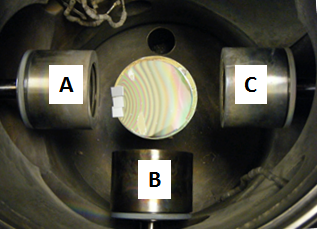
\includegraphics[width=0.6\textwidth]{chapter_2/fenris2}
\caption{Off-axis configuration of the guns enable combinatorial studies of thin film amorphous oxides. Up to three sputtering guns can be energized simultaneously to form a ternary composition. RF biases are applied to the substrate to form a dense film.}
\label{fenris2}
\end{figure}

Here, off-axis means the target face is oriented perpendicular to the sample surface. Deposition from a single target in this configuration results in a natural thickness gradient across the wafer due to the exponential decrease in deposition rate with distance. Thus, when multiple sputtering guns are active a natural composition gradient is obtained. Because of the intimate intermixing of the sputtered constituents, the compositional resolution that can be achieved is typically better than $<$ 0.1 mole-$\%$. Note, the chamber is capable of sputtering in the conventional ``on-axis" configuration as well, where the target face is oriented parallel to the sample surface. This orientation was preferred when single composition films of uniform thickness was required.

Base pressures down to 10$^{-6}$ Torr were achieved by using a turbo molecular pump that is backed by a roughing pump. A gate valve is throttled to control the chamber pressure during deposition. Film thicknesses generally varied from approximately 10 to 300 nm. An rf bias was often applied to the films during off-axis deposition to preclude the formation of voidy films. These voids have been shown to exhibit defect mediated polarization mechanisms that are undesirable for material integration into practical devices \cite{Barron2009}. Once the films were deposited the samples were transferred back to the evaporation chamber. This time, 300 \AA\;Pt dots were deposited onto the sample by evaporation through a shadow mask with 200 $\mu$m diameter holes arranged in a square array with center to center spacing of 500 microns. 

\subsection{Application of e-beam evaporation of metal electrodes and electrode material choices}

E-beam evaporation is a technique that uses high energy electron beams to evaporate source materials in a vacuum. Typically the evaporators are encased in a bell jar, and evacuated to $\sim$ 10\textsuperscript{-7} Torr prior to deposition. A large current is passed through a metal filament causing electrons to boil off thermionically and accelerate towards the source material, which is resting inside a water cooled hearth. The electrons are steered by the magnetic field produced by a solenoid. The force on the electron can be calculated using the Lorentz force equation, $\textbf{F} = q_{e}\textbf{E} + q_{e}\textbf{v} \times \textbf{B}$. The field can also be modulated so that the electron beam rasters across the source material, improving deposition uniformity. The main advantage over thermal evaporation is that e-beam evaporation can be used to evaporate most any material, even highly refractory metals. Although the energy input of the electron beam on the source material far exceeds the strength of the chemical bonds of the material, the overall process is still thermal. Thus the atoms are deposited with energy of $\sim$ 0.2 eV. The fact that it is a line of sight process is also favorable for the use of a shadow mask and minimizing the formation of penumbra caused by insufficient shadowing.  

Some consideration is required when choosing the material that is to be used as electrodes. Because we are measuring the electrical properties of thin film amorphous oxides using MIM structures, we would like to minimize the amount of interfacial oxide formation that would result in inaccurate characterization of the thin film. As an electrode material, platinum is an obvious choice because it is a chemically inert material. However, silicon has a native surface oxide that inhibits the direct deposition of noble metals such as Au and Pt directly onto Si because of their different bonding characteristics. In such a case, a metal that is chemically more reactive needs to be deposited beforehand as an adhesion layer. In this study, a 300 \AA\;layer of Cr was commonly used, but other ``reactive" metals such as Ti would also suffice. A thickness of 300\;\AA\;is more than enough material to yield a continuous layer. 
	
\subsection{Reactive radio frequency magnetron sputtering and the co-sputtering technique}

Sputtering, like e-beam evaporation, is an energy vaporization method, making it suitable for depositing a wide range of materials. However, evaporation is a thermal process, whereas sputtering involves momentum transfer of partially ionized gas particles in the form of a plasma. Conservation of energy and momentum tells us that if two particles are of similar mass, then only a small amount of energy is required to displace the particles from their rest state. For this reason, inert gases such as Ar, Kr, and Xe are suitable choices as impinging particles because of their comparable masses to the target elements. Furthermore, they are generally inexpensive and high in purity. For this study, we used Ar---specifically Ar\textsuperscript{+}---as the impinging gas.

Energy input of ionized gas ions in sputtering usually ranges from 10 to a few 100 eV. Low energy ions can be used for surface modification or densification of films \cite{Coburn1972, Huang2010}, while higher energies are required for sputtering. Dislodged (sputtered) target atoms typically acquire kinetic energies up to several electron volts and undergo various reactions such as colliding with reactive gasses (reactive sputtering), generating secondary electrons before eventually condensing onto the substrate. The final structure and morphology of the thin film ultimately depends on several tunable parameters. 

Structural control can be achieved using various flavors of sputtering. In our study we mainly use rf magnetrons. Rf sputtering is a flexible technique that can be used to deposit from both metals and insulating targets. Sinusoidal power is applied to the driven electrode, with frequency of oscillation typically at 13.56 MHz. Initially during the positive half of the cycle, the electrons respond to the electric field and are drawn to the cathode. However, when the electrode is driven negative, the ions are unable to respond to the sudden change in electric field due to their large size. Thus, the amount of ion current that flows through the target is significantly smaller in comparison to the electron current. Flow of excess electron current is most often impeded by the use of a blocking capacitor. As time progresses the power and the coupling capacitor continues to charge negatively (almost instantaneously). Eventually a steady state is reached and the target is negatively self-biased. Maximum power delivery to the target is accomplished by means of a matching network that works in parallel with the blocking capacitor. 

Use of planar magnetron sputtering guns instead of planar-diode further improves sputtering efficiency. Powerful circular magnets embedded in planar magnetron guns produce magnetic field lines that emanate out into the chamber and curl around back into magnets at the center of the gun. When an electric field is simultaneously applied across the planar cathode, it creates a region where the electric and magnetic fields cross perpendicularly. Electrons in this region travel in a cycloidal pattern and become confined to that region. Consequently, ionization of gas atoms is most efficient there, producing a circular race-track erosion pattern. Magnetron sputtering has the effect of nonuniform erosion patterns across the target surface, but only requires a low working pressure to sputter materials. Therefore the deposition rate is increased due to decreased collisions and lower voltage requirements to sustain the plasma due to the confinement of electrons. 

Most films in this study were sputtered reactively; films were deposited from metal targets in the presence of a working and reactive gas. The gaseous cocktail consisted of Ar as our working gas and O$_{2}$ as the reactive component. Reactive sputtering has several advantages over sputtering directly from a compound (ceramic) target. For one, metal targets can be sputtered at a higher deposition rate compared to ceramic targets and are not as brittle and prone to thermal shock. Higher target purity is also achievable with metal targets so in theory the deposited films should be of higher purity. However, because the target atoms must undergo reactions with the reactive gas to form compounds, in practice one has to consider appropriate partial pressures and gas compositions ratios during deposition to ensure stoichiometric deposition from a metal target. This can be done by controlling the working pressure of the deposition chamber during sputtering, and also by changing the flow rate of the gasses using a mass flow controller.


\section{Characterizing dielectric properties}
\subsection{Capacitance measurements}

Capacitance measurements were performed using a semi-automatic probe station controlled by Labview software, capable of mapping the capacitance and dissipation of an entire 3 inch wafer. Contact to the Pt top electrode was made using a BeCu probe tip, while gold wire was soldered to an exposed portion of the Pt bottom electrode with indium. The probe and gold wire are both connected to a Hewlett Packard 4284A inductance-capacitance-resistance meter (LCR) with a stripped coaxial cable. The LCR meter works by applying AC voltage ($V$) and recording the current ($I$) which is used to calculate the capacitance and dissipation factor based on their phase relation. In this study, the applied AC voltage was on the order of 100 mV.

Both current and voltage are complex quantities and thus can be expressed as complex exponentials with phase lag $\theta$ between the two quantities,   
\begin{equation}\label{eq:I}
V = \vert V\vert e^{j\omega t}
\end{equation}
\begin{equation}\label{eq:V}
I = \vert I\vert e^{j(\omega t + \theta)}.
\end{equation}
In an ideal capacitor the current leads the voltage by $\pi/2$ so any deviation from this value is symptomatic of a non-ideal (real) capacitor. As discussed earlier, the impedance of a real capacitor has contributions from lossy and non-lossy components. Hence, the ratio between the current and voltage is the complex impedance and can be expressed in the following way:
\begin{equation}\label{eq:cap}
\frac{V}{I} = Z = R + jX_{c}.
\end{equation}
Here, $R$ represents the real portion of the impedance (resistance), $X_{c}$ is the imaginary component known as the reactance, and $j$ is the imaginary number $j = \sqrt{-1}$. We can represent the quantity Z as a vector composed of real and imaginary components $R$ and $X_{c}$ as in Figure \ref{fig:compleximpd}.

\begin{figure}[ht]
\centering
\noindent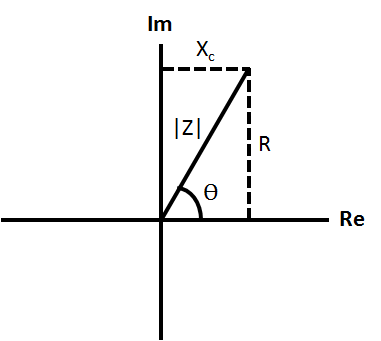
\includegraphics[width=0.5\textwidth]{chapter_2/compleximpedance}
\caption{Complex impedance.}
\label{fig:compleximpd}
\end{figure}

The magnitude of the impedance $\vert Z\vert$ and angle $\theta$ denoting the phase difference between $R$ and $X_{c}$ is,    
\begin{equation}\label{eq:magZ}
\vert Z\vert = \sqrt{R^{2} + X_{c}^2}
\end{equation}
\begin{equation}\label{eq:thetaZ}
\theta = \tan{\left(\frac{X_{c}}{R}\right)}^{-1}
\end{equation}
For mathematical simplicity, it is convenient to write the impedance as admittance $Y$, which is just the inverse of $Z$,
\begin{equation}\label{eq:admit}
\frac{1}{Z} = Y = G + jB_{c}
\end{equation}
such that now $\vert Z \vert$ and $\theta$ are 
\begin{equation}\label{eq:magD}
\vert Z\vert = \sqrt{G^{2} + B_{c}^2}
\end{equation}
\begin{equation}\label{eq:thetaD}
\theta = \tan{\left(\frac{G}{B_{c}}\right)}^{-1}
\end{equation}
in which $G$ is known as the conductance and $B_{c}$ is the susceptance with value $\vert\omega C\vert$. Therefore, the dissipation factor D is, 
\begin{equation}\label{eq:tand}
D = \tan{\delta} =  \tan{\frac{\vert\omega C\vert}{G}}
\end{equation}
and is related to $\theta$ by $\delta = \pi/2 - \theta$. Finally, since we known the film thickness and contact area of the metal electrodes in the MIM capacitors, we can use the measured capacitance to calculate the dielectric constant using equation \ref{eq:cap2}.

\subsection{Optical measurements}

At optical frequencies the atomic nuclei are too sluggish to respond to the alternating electric field, thus only the electronic response contributes significantly to the relative permittivity. The dielectric response at optical frequencies is expressed as the complex refractive index $\tilde{n} = n + ik$, which is a complex quantity written in terms of the absorption coefficient $k$, and $n$, the ratio between the speed of light in a vacuum and the speed of light in a medium. We can determine $n$ and $k$ as well as geometric properties such as film thickness by conducting optical measurements; in our case we use variable angle spectroscopic ellipsometry (VASE). 

Ellipsometry works by shining light onto the surface of the material and measuring the change in polarization of the light after it has interacted with the material. For a single interface, we can quantify the polarization of the light in terms of the Fresnel reflection coefficients ($r_{p}$) and ($r_{s}$), the p and s-polarization components, respectively
\begin{equation}
r^{p}_{12} = \frac{\tilde{N_{2}}\cos{\phi_{1}} - \tilde{N_{1}}\cos{\phi_{2}}}{\tilde{N_{2}}\cos{\phi_{1}} + \tilde{N_{1}}\cos{\phi_{2}}}
\qquad
r^{s}_{12} = \frac{\tilde{N_{1}}\cos{\phi_{1}} - \tilde{N_{2}}\cos{\phi_{2}}}{\tilde{N_{1}}\cos{\phi_{1}} + \tilde{N_{2}}\cos{\phi_{2}}}.
\label{eq:fres}
\end{equation}
In the equation, $\tilde{N_{1}}$ and $\tilde{N_{2}}$ denote the complex refractive index of materials 1 and 2, and $\phi_{1}$ and $\phi_{2}$ are the angle of incidence and transmission from medium 1 to medium 2, respectively. Now, to describe a two interface material the total reflection coefficients for the p and s-polarized components $R_{p}$ and $R_{s}$ can be explicitly written as, 
\begin{equation}
R^{p} = \frac{r^{p}_{12}+r^{p}_{23}e^{-j2\beta}}{1+r^{p}_{12}r^{p}_{23}e^{-j2\beta}}
\qquad
R^{s} = \frac{r^{s}_{12}+r^{s}_{23}e^{-j2\beta}}{1+r^{p}_{12}r^{s}_{23}e^{-j2\beta}}.
\label{eq:refcof}
\end{equation}
The subscripts denote the incident medium and transmitted medium, while $\beta = 2\pi \frac{d}{\lambda}\tilde{N_{2}} \cos{\phi_{2}}$ describes the phase shift of the light that occurs when passing through the various mediums. 

We can combine these quantities in the fundamental equation of ellipsometry
\begin{equation}
\frac{R_{p}}{R_{s}} = \tan{(\psi)}e^{i\Delta}.
\label{ref:ellipsometry}
\end{equation}
The amplitude ratio of reflection, $\tan{(\psi)}$,  and phase shift, $\Delta$, can be measured experimentally, however relevant optical and geometric parameters such as film thickness and refractive index are calculated by fitting to a model. Note, the variability of the angle and the spectroscopic nature of the measurement increases the number of fitted parameters, making the fitting process  more robust. For many optically transparent non-absorbing materials---oxides being one of them---the Cauchy relation provides a simple empirical solution. The Cauchy dispersion relation is,
\begin{equation}
n = A + \frac{B}{\lambda^{2}} + \frac{C}{\lambda^{4}}.
\label{eq:cauchy}
\end{equation}
The capital letters are fitted parameters and $\lambda$ is the wavelength of light. For most materials a two term model (one utilizing only parameters $A$ and $B$) is enough to fully describe the dispersion relation of the material. The recursive fitting procedure is performed in the VASE software package provided by Woollam Inc.  

\section{Characterizing film composition and density}
\subsection{Determining film composition}
Determining the composition dependent properties of the oxides hinges on accurate characterization of film composition. We relied on two methods: the first is to simply infer the composition profiles based on deposition rate calibrations, while the second is a direct measurement of the film composition using wave length dispersive spectroscopy (WDS).

Deposition rate calibrations were obtained by depositing elemental oxide films in the off-axis configuration onto a bare 3" Si wafer. Depositions typically lasted 20 minutes, although in some cases were extended if the deposition rate of the oxide was low. All depositions were eventually normalized to deposition rates (thickness/unit time) to account for the variability in deposition time. A bias of -75 V was applied to the substrate during calibration runs to emulate the deposition conditions of cosputtered films at room temperature.

The majority of the films studied were binary oxides thus requiring only linear thickness profiles across the diameter of the wafer (thickness measured using ellipsometry). This corresponds to a profile that starts from the center of the sputtering target and extends perpendicular to the target face (Figure \ref{calibration}).
\begin{figure}
\centering
\noindent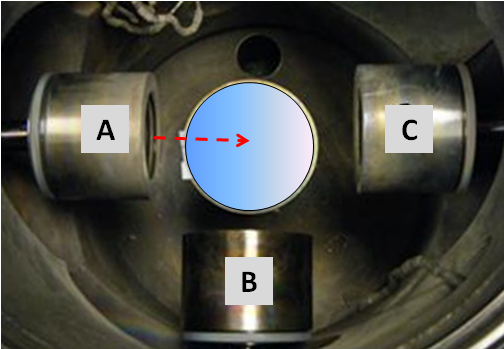
\includegraphics[width=0.7\textwidth]{chapter_2/calibration}
\caption{Guns in the off-axis configuration for deposition rate calibration. Figure depicts a deposition profile along Gun A.}
\label{calibration}
\end{figure}
Three to four equally spaced points on the wafer that are collinear to this line were sufficient to generate an accurate linear thickness profile. An exponentially decaying function was fit to the measured thickness to obtain decay length and thickness at substrate edge. To determine the composition ratio of a binary oxide, we must first convert the thicknesses to molecules per unit area for each elemental oxide using the following equation,
\begin{equation}\label{eq:composition_a}
[A_{x}O_{y}] = t(A_{x}O_{y})*\text{A.M.}(A_{x}O_{y})*\rho (A_{x}O_{y})*N_{a}.
\end{equation}

For elemental oxide $A_{x}O_{y}$,  $t(A_{x}O_{y})$ denotes the thickness from the linear profile, $\text{A.M.}(A_{x}O_{y})$ is the atomic mass of the molecule, $\rho (A_{x}O_{y})$ is the density of the molecule, and $N_{a}$ is Avogadro's number. Once the number of molecules per unit area is determined, the composition ratio of molecule $A_{x}O_{y}$ can be inferred by simply taking a ratio,
\begin{equation}\label{eq:composition_b}
\frac{[A_{x}O_{y}]}{[B_{p}O_{q}]+[A_{x}O_{y}]}
\end{equation}
in which the numerator represents the number of $A_{x}O_{y}$ molecules per unit area, whereas the denominator is the total number of molecules per unit area. The area term automatically cancels out since it is present in both the numerator and denominator. The ratio is only valid when the deposition times are consistent for each calibration.

Although composition profiles are typically highly reproducible (to $\sim$1 at\%), the conditions in the chamber may slightly change day to day affecting film properties between runs, so it is still instructive to perform a direct composition measurement; for this we use WDS. WDS is a sister technique to the EDS (energy-dispersive x-ray spectroscopy) and relies on the interaction of electrons with the material to stimulate emission of x-rays. The emitted x-ray energies are characteristic to the material and therefore in theory, the composition ratios can be discerned.

In comparison to EDS, WDS has a much higher spectral resolution; the resolution of EDS is typically on the order of $\sim$ 100 eV, while WDS can resolve peaks down to several eV at full width half max (FWHM) \cite{Goldstein2003}. Improved resolution in WDS is achieved by preferential diffraction of characteristic x-rays through an analyzing crystal, in which the interaction of the x-rays with the crystal is dictated by Bragg's law, $n\lambda = 2d\sin(\theta)$. The detector, which collects the diffracted x-rays, and the crystal are simultaneously moved such that angle $\theta$ is varied by changing the position of the detector relative to the sample. Varying $\theta$ in turn selects which wavelength is diffracted according to Bragg's law. 

WDS's accuracy is further improved by the use of standards with known composition. The task now is to take the measured intensity from the sample for element $i$, ${I_{i}}$, and compare it to the intensity measured from the standard ${I_{(i)}}$ to determine the composition in the sample. As a first approximation, one can determine the ``k ratio,"
\begin{equation}\label{eq:kratio}
\frac{C_{i}}{C_{(i)}} = \frac{I_{i}}{I_{(i)}} = k_{i}
\end{equation}
which assumes that the ratio between ${I_{i}}$ and ${I_{(i)}}$ determines the mass composition ratio $C_{i}$/$C_{(i)}$, the composition fraction of the element of interest in the sample, and the composition fraction of the element of interest in the standard, respectively. Complicating the analysis are ``matrix effects," e.g. absorption and fluorescence, which have to be taken into account since they lead to errors in the k-ratio. Matrix effects are divided into three effects: atomic number ($Z_{i}$), x-ray absorption ($A_{i}$), and x-ray fluorescence ($F_{i}$). We can obtain the corrected k ratio by multiplying the correction factor for element $i$,
\begin{equation}\label{eq:zaf}
k(\text{corrected})_{i} = k_{i} [ZAF]_{i}.
\end{equation}

\subsection{Measuring film density using x-ray reflectivity}

To calculate the polarizability of the material using the Clausius-Mossotti relation one needs to know the dielectric constant, $\varepsilon_{r}$, and density, $\rho$. While the dielectric constant is easily determined by C-D measurements, the density of an amorphous material is more difficult to ascertain, particularly since we require a systematic evaluation of $\rho$ as a function of composition (position on the wafer). For our study, we rely on x-ray reflectivity (XRR) measurements to probe the density of the material at various points on the wafer. 

X-ray reflectivity works by total external reflection, which occurs when x-rays are shined on a material with an angle of incident ($\theta$) that is less than the critical angle $\theta_{c}$---where the critical angle is typically $\theta_{c}$ $<$ 0.5. Total external reflection only occurs because the refractive index, $n$, of a material is less than one at x-ray wavelengths. Because the condition for total external reflection depends on the electron density of the material, and therefore mass density, measuring the critical angle is an indirect measurement of material density. 

Reflectivity measurements were carried out using the Rigaku Smartlab diffraction system. Sample alignment is crucial to XRR measurements, hence we aligned the sample at each point on the wafer prior to each measurement. Standard 40 keV Cu K-$\alpha$ X-rays were conditioned through a slit assembly to minimize the beam footprint (footprint $\leq$ 10mm$\times$3mm). Note, a large beam footprint is undesirable since we want to minimize the compositional averaging from the sample. In some cases a Ge (220)$\times$2 monochromator was utilized to further minimize the beam footprint. The reflected x-rays were further conditioned by the receiving slit assembly before being collected by the detector. To simplify the analysis, we took the critical angle to be the angle in which the intensity becomes half the total reflected intensity \cite{Parratt1954}. The critical angle is related to the mass density by the following formula 
\begin{equation}
\rho = \frac{\theta_{c}^{2}\pi A}{Zr_{e}\lambda^{2} N_{A}} 
\label{eq:rho}
\end{equation}
where $A$ is the atomic mass unit, $r_{e}$ the classical electron radius, $\lambda$ the x-ray wavelength, $N_{A}$ is Avogadro's number, and $Z$ the atomic number \cite{Bahr1993}. Intrinsic to this equation is the assumption that $\theta_{c} = \sqrt{2\delta}$, which requires that the atomic form factor $f^{0}_{1}$ $\approx$ $Z$ and that  $f^{0}_{2} << f^{0}_{1}$. These are fairly reasonable assumptions to make at these x-ray energies \cite{Chantler1995}.

\section{Structural characterization of non-crystalline materials}

The Merriam-Webster Webster dictionary defines the word amorphous as "having no definite form," suggesting that amorphous materials lack any kind of ordering. However, this is far from the truth. In fact, amorphous materials consist of recurring structural elements that exhibit ordering in short range (typically several nearest neighbor distances). The complexity of the matter is evidenced, for example, by the on-going debate over the structural topology of amorphous Si \cite{Treacy2012}. The fact is, it merely appears that amorphous materials lack ordering because conventional methods that probe structure (e.g. x-ray diffraction using Cu-K$\alpha$ radiation) are typically not able to uncover short or even medium range order. Therefore, researchers must rely on more specialized methods \cite{Cockayne2007} to unravel the ``hidden" structure of amorphous materials. 

\subsection{Real space diffraction}

We rely heavily on several preexisting techniques that have experienced historic development, one of which is real space diffraction analysis. The goal of the technique is to determine a pair distribution function (PDF), $g(r)$, that represents the probability of finding an atom at distance $r$ from an origin atom. Several references on this topic are available \cite{Billinge2003,Warren1990,Waseda1980, Farrow2009}. To obtain $g(r)$ we must compute $\varphi(Q)$, the reduced intensity function from measured X-ray intensities, $I(Q)$, and then apply a sine Fourier transform. The canonical expression of the PDF is,
\begin{equation}\label{eq:PDF}
g(r) =\rho_{a} + \frac{1}{2\pi^{2}r} \int_{0}^{\infty} \varphi(Q)\sin{Qr}\;dQ.
\end{equation} 
Binary alloys require further mathematical treatment (to extract partial distribution functions for proper structural analysis), and ternary even more so. Recent improvements in computational power allow modeling of complex amorphous systems with great accuracy \cite{Petkov1998, Bassiri2011}, and can be used in conjunction with experimental data to determine partial distribution functions. In the following section we derive the PDF for the simple case of a single element system, similar to the derivation found in \cite{Warren1990}.  

In the kinematical limit the scattering intensity is written as the sum of amplitudes from different atoms multiplied by its complex conjugate. Defining a difference vector $\textbf{r}_{ji} = \textbf{r}_{j} - \textbf{r}_{i}$:
\begin{equation}\label{eq:ScatI}
I(Q) = \sum_{j}\sum_{i} f_{j}f_{i} e^{(2\pi i/\lambda) (\textbf{s}-\textbf{s}_{0}) \cdot \textbf{r}_{ji}}.
\end{equation}
We can separate the sums for terms where $i=j$
\begin{equation}\label{eq:Ic1}
I(Q) = \sum_{j}f^{2}+ \sum_{j}f^{2}\sum_{i\neq j} e^{(2\pi i/\lambda) (\textbf{s}-\textbf{s}_{0}) \cdot \textbf{r}_{ij}}.
\end{equation}
Introducing a density function $g_{j}(\textbf{r}_{ij})$ we can write the the sum for the $i\neq j$ term as an integral over the volume element $dV$
\begin{equation}\label{eq:Ic2}
I(Q) = \sum_{j}f^{2}+ \sum_{j}f^{2}\int g_{m}(\textbf{r}_{ij})e^{(2\pi i/\lambda) (\textbf{s}-\textbf{s}_{0}) \cdot \textbf{r}_{ij}}dV.
\end{equation}
Adding and subtracting the average atom density in the sample $\rho_{a}$, we obtain two integrals over the sample volume:
\begin{equation}\label{eq:Ic3}
I(Q) = \sum_{j}f^{2}+ \sum_{j}f^{2}\int [g_{m}(\textbf{r}_{ij})-\rho_{a}]e^{(2\pi i/\lambda) (\textbf{s}-\textbf{s}_{0}) \cdot \textbf{r}_{ij}}dV + \sum_{j}f^{2}\int \rho_{a}e^{(2\pi i/\lambda) (\textbf{s}-\textbf{s}_{0}) \cdot \textbf{r}_{ij}}dV.
\end{equation}
To solve the integral we take an orientational average over the volume of the sample, assuming an isotropic distribution of atoms. The average density function is $g(\textbf{r}) = \langle g_{j}(\textbf{r}_{ij})\rangle$, in which $\textbf{r} = \textbf{r}_{ij}$ for fixed atom displacements. We consider amorphous materials of the type such that for large $\textbf{r}$ values, $g(\textbf{r}) - \rho_{a}$ goes to zero. We can thus simplify the sum of the self-scattering terms by replacing the sum with $N$. Also, the third term only contributes to I(Q) at small scattering vectors, so it can be dropped from the equation if small angles are not included in the data. Substituting the scattering vector $Q = 4\pi \sin{\theta/\lambda}$, and from the fact that 
$(\textbf{s} - \textbf{s}_{o})\cdot(\textbf{r}_{nm}) = 2\sin{\theta}\;r\cos{\phi}$, we can solve the integral in equation \ref{eq:Ic3}
\begin{equation}\label{eq:Ic4}
I(Q) = Nf^{2}+ Nf^{2}\int^{\infty}_{0}\int^{\pi}_{0}[g(r)-\rho_{a}] e^{ikr\cos{\phi}}2\pi r^{2} \sin{\phi}\;d\phi\;dr
\end{equation}
\begin{equation}\label{eq:Ic5}
I(Q) = Nf^{2}+ Nf^{2}\int^{\infty}_{0} 4\pi r^{2}[g(r) - \rho_{a}] \frac{\sin{kr}}{kr}\;dr.
\end{equation} 
To get the PDF we introduce the reduced intensity function $\varphi(Q)$
\begin{equation}\label{eq:RIF}
\varphi(Q) = \left[\frac{I(Q) - Nf^{2}(Q)}{Nf^{2}(Q)}\right]Q
\end{equation}
which gives us, 
\begin{equation}\label{eq:phi}
\varphi(Q) = 4\pi\int^{\infty}_{0}  r[g(r) - \rho_{a}] \sin{kr}dr.
\end{equation}
Currently phi is a function of Q-space. The PDF is a real space function and therefore, we need to apply a Fourier transform to $\varphi(Q)$. Defining $f(r) =  r[g(r) - \rho_{a}]$, we obtain the following Fourier pair:
\begin{equation}\label{eq:pair}
\begin{split}
 & \varphi(Q) = 4\pi\int^{\infty}_{0} f(r) \sin{kr}\;dr\\
 & f(Q) = \frac{1}{2\pi^{2}}\int^{\infty}_{0} \varphi(Q) \sin{kr}\;dr.
\end{split}
\end{equation}
From this we see that with a little rearranging, one can easily obtain the result presented in equation \ref{eq:PDF}.
Experimentally, the challenge lies in accurately measuring the scattered intensity $I(Q)$ and applying the proper correction algorithms such that an accurate PDF can be obtained. All diffraction spectra in this study were obtained at the Cornell High Energy Synchrotron Source (CHESS) A2 line at 40keV, corresponding to an x-ray wavelength of 0.030657 nm.

\subsection{Silicon nitride membranes for x-ray diffraction}

*Silicon nitride membranes were designed and fabricated by Lauren Taylor*

\noindent The signal from the silicon diffuse scattering adds an extra step in the data reduction process when characterizing thin films deposited on single crystal silicon in transmission \cite{Gregoire2009a}. For amorphous materials, this extra signal from silicon diffuse scattering is especially problematic since the captured signal from the amorphous materials are not as intense in comparison to crystalline materials. To circumvent this problem altogether, we mainly performed scattering experiments on films that were deposited on amorphous silicon nitride membranes. Because the nitride membranes are thin (a few microns thick) and amorphous, the subtraction process can be performed with greater ease.

Silicon nitride membrane arrays were fabricated using standard clean room processes in Cornell's Nanofabrication Facility (CNF). The membranes were arranged in a two-dimensional array as shown in Figure \ref{windows}. 
Window size was modified depending on the number of membranes in the array. The windows for the 12$\times$12 array were 2 mm on each side, whereas the windows for the 8$\times$8 and 9$\times$9 arrays were 3 mm.

\begin{figure}
\centering
\noindent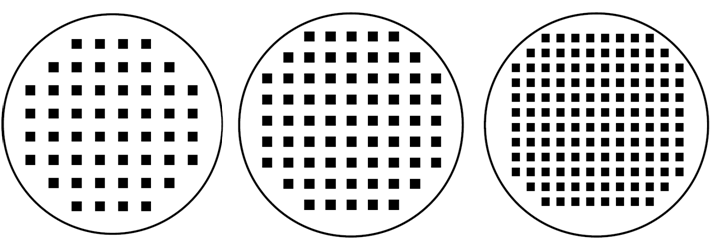
\includegraphics[width=\textwidth]{chapter_2/windows}
\caption{Cartoon showing the different silicon nitride membrane arrays used for the diffraction studies. From left to right: 8$\times$8, 9$\times$9, and 12$\times$12 arrays.}
\label{windows}
\end{figure}

Prior to silicon nitride deposition, 3 inch double-side polished wafers were cleaned in an acid bath followed by a base bath and rinsed in deionized water after each. The wafers were then transferred to an MRL Industries low pressure chemical vapor deposition (LPCVD) furnace where low stress silicon nitride was deposited. The nitride deposition rate was approximately 30 \AA\;per minute determined from prior calibration runs. The substrates were kept in the furnace for 7 hours at 775 \textdegree C, which yielded nitride films that were approximately 1.5-1.6 microns thick determined by reflectometry (FilMetrics Film Measurement System). Window array patterns were developed on the wafer using standard photolithographic methods. This involves transferring a photoresist pattern of the array onto the nitride coated substrate and etching away the nitride in the exposed windows. Finally, the wafer was back-etched using a potassium hydroxide solution forming the silicon nitride windows.

\subsection{From measured intensity to PDF}

Data acquisition is only half the battle, the other being data reduction and analysis. To refine the raw data into something we can analyze, we first normalized to the total x-ray flux (IC3 counts) and subtracted the silicon nitride background from the raw 2D spectra. The spectra was then collapsed into a 1D diffraction pattern by integrating azimuthally in fit2D \cite{Hammersley1996}.

At this point it is common to apply further corrections to the diffraction pattern. This includes polarization, absorption, multiple scattering effects, etc., and have been widely implemented in several PDF analysis programs \cite{Qiu2004}. However, it is fairly time consuming to master these programs and careful consideration of the various errors in diffraction analysis is required, calling on a high level of expertise. In this study we make use of a less arduous approach by analyzing the data \emph{ad hoc}. 

The \emph{ad hoc} approach is possible because of certain general properties of the structure function. Corrections to measured intensity, $I_{m}(Q)$, are expected to be  either additive or multiplicative,
\begin{equation}
I_{c}(Q) = a(Q)I_{m}(Q) + b(Q)
\label{eq:Im}
\end{equation}
where $a(Q)$ and $b(Q)$ are the Q dependent multiplicative and additive factors to the measured intensity, which if varied appropriately, gives us the correct form of the coherent scattered intensity, $I_{c}(Q)$. The correction factors can also be related to the total scattering structure function $F(Q)$ (as denoted by some researchers), essentially equivalent to $\varphi(Q)$ found in Equation \ref{eq:RIF}
\begin{equation}
F(Q) = \alpha(Q)I_{m}(Q) + \beta(Q).
\label{eq:F{Q}}
\end{equation}
The critical insight is that although $\alpha(Q)$ and $\beta(Q)$ are not known \emph{a priori}, the general form and behavior of the correction factors are known. Hence, the correct forms of $\alpha(Q)$ and $\beta(Q)$ can be determined variationally using PDFgetX3 \cite{Juhas2013a}.

We feed the background subtracted diffraction patterns into PDFgetX3 using the Python based command-line interpreter \cite{Juhas2013a}. The program then variationally adjusts the correction factors and applies a sin Fourier transform to $F(Q)$ to solve for the PDF:
\begin{equation}\label{eq:pdf}
g(r) = \frac{2}{\pi} \int_{Q_{min}}^{Q_{max}} F(Q) \sin{Qr} dQ.
\end{equation}
Note, that because we cannot collect data to infinite wavelengths, $Q_{max}$ is always a finite value. This is equivalent to convolving a step function beyond $Q_{max}$, which becomes convolved with the data, resulting in ``truncation" errors. In order to reduce this error, researchers typically collect data to sufficiently large Q values to incorporate a large number of Fourier components to perform the transform \cite{Dykhne2011}.

Direct information such as bond distance and coordination number are immediately available from the refined PDF. As mentioned earlier a more involved, but illuminating approach is simulating the amorphous structure \cite{Zhang2007, Bassiri2011}. This enables us to not only confirm what we learn from the direct analysis, but also ascertain additional information such as the partial distribution functions for multicomponent systems and electrical properties such as the dielectric constant.

\subsection{X-ray absorption fine structure}

The PDF method provides us with valuable local structural information. Nonetheless, the technique is not element specific. X-ray absorption fine structure (EXAFS, or XAFS)---a method which falls under X-ray absorption spectroscopy (XAS)---is an \emph{element specific} local probe of the material, which can be used to extract information much like the PDF method and further, gather chemical information about the material such as the valence state of an element. 

EXAFS capitalizes on the wave-particle behavior of electrons. Within the x-ray energies we are interested in (1 $\leq$ E $\leq$ 100 keV), x-rays are absorbed by the photoelectric effect. Absorption of the x-ray excites an electron out of the atom leaving a core-hole. The element specificity is achieved by tuning the energy of the x-ray such that we only look at the absorption event for a specific element. Several events can also follow the absorption process such as the annihilation of the core-hole via fluorescence, or the emission of an Auger electron through an Auger process. The absorption of the x-ray results in the attenuation of the original x-ray intensity, $I_{o}$ to $I$, which is measured by the detector. The relation between $I_{o}$ and $I$ can be expressed by the Beer-Lambert law 
\begin{equation}
I = I_{o}e^{-\mu(E) t}
\label{eq:BL}
\end{equation}
in which the absorption coefficient $\mu(E)$ is also an energy dependent quantity. The presence of neighboring atoms scatters the emitted photo-electron and in this process interferes with other scattered photo-electrons. This interference effect produces fringing in the absorption coefficient known as the ``fine structure," which provides information about the local environment in the material. We can write the fine structure in terms of the absorption coefficients,
\begin{equation} 
\chi(E) = \frac{\mu(E) - \mu_{o}(E)}{\Delta\mu_{o}(E_{o})}
\label{eq:EXAFS_chi}
\end{equation}
where $\mu_{o}(E)$ is the background absorption and $\Delta\mu_{o}(E_{o})$ is the edge step which normalizes the equation to one absorption event. We can extract useful information from the data by modeling the fine structure. Taking into account inelastic and multiple scattering and thermal vibrations the EXAFS equation is
\begin{equation} 
\chi(k) = \sum_{i}\frac{N_{i}S_{o}^{2}f_{i}e^{-2R_{i}/\lambda(k)}e^{-2k^{2}\sigma_{i}^{2}}}{kR^{2}_{i}} \sin{2kR_{i} + \delta_{i}(k)}.
\label{eq:exafs2}
\end{equation}
Here, we have expressed the EXAFS as a function of the photo-electron wave number $k = \sqrt{\frac{2m(E-E_{o})}{\hbar}}$. By fitting to the EXAFS equation, we can extract information such as bond distance and coordination number centered around a specific element. 

All EXAFS experiments were carried out in CHESS's F3 line. We tuned the energy of the x-rays to the desired absorption edge (Ta L-3 absorption edge for tantalum based materials which sits at $\sim$9883 eV). Ta metal foil was also used to calibrate the absorption edge. Data reduction and analysis was performed using the ATHENA and ARTEMIS software packages \cite{Ravel2005}.
